\documentclass[table]{article}
% For math environments
\usepackage{amsmath, amsfonts}
% For links
\usepackage[hidelinks]{hyperref}
% So space it put between paragraphs
\usepackage{parskip}
% For figures
\usepackage{tikz}
% Set the margins to not be ridiculous
\usepackage[margin=0.75in]{geometry}
% For multiple columns
\usepackage{multicol}
% For controlling enum/itemize spacing and indentation
\usepackage{enumitem}

% For tikz plots
\usepackage{pgfplots}
% This isn't needed but avoids a compiler warning
\pgfplotsset{compat=1.16}

% Allow multi-line equations to be broken across pages
\allowdisplaybreaks

% Use @ as a letter
\makeatletter

% Scale down all tikz coordinates while maintaining font size
\tikzset{every picture/.style={scale=0.45, every picture/.style={}}}


% Macros
% Monospace code
\def\code#1{\texttt{#1}}

% Greek letters
\def\a{\alpha}
\def\b{\beta}
\def\g{\gamma}
\def\d{\delta}
\def\D{\Delta}

% Some common sets
\def\es{\varnothing}
\def\ints{{\mathbb{Z}}}

% Commands that make life easier
\newcommand\gath[1]{\begin{gather} #1 \end{gather}}
\newcommand\gaths[1]{\begin{gather*} #1 \end{gather*}}
\newcommand\ali[1]{\begin{align} #1 \end{align}}
\newcommand\parens[1]{\left( #1 \right)}
\newcommand\squares[1]{\left[ #1 \right]}
\newcommand\braces[1]{\left\{ #1 \right\}}
\newcommand\angles[1]{\left\langle #1 \right\rangle}
\newcommand\deriv[2]{\frac{d #1}{d #2}}
\newcommand\abs[1]{\left| #1 \right|}
\newcommand\floor[1]{\left\lfloor #1 \right\rfloor}
\newcommand\ceil[1]{\left\lceil #1 \right\rceil}
\DeclareMathOperator{\lcm}{lcm}
\def\non{\nonumber \\}
\newcommand\unit[1]{~\mathrm{#1}}
\newcommand\combos[2]{{}_{#1}C_{#2}}

% Set stuff
\def\ss{\subseteq}

% Multiline equation space
\def\mlesp{\hspace{1.2cm}}

% For grid diagrams
\newcommand\gridbox[3]{\draw (#1,#2) rectangle (#1+1,#2+1) node[pos=.5] {#3};}
\newcommand\gridboxh[3]{\draw[fill=red!20] (#1,#2) rectangle (#1+1,#2+1) node[pos=.5] {#3};}
\newcommand\gridboxb[3]{\draw[fill=black] (#1,#2) rectangle (#1+1,#2+1) node[pos=.5] {#3};}
\newcommand\gridsym[3]{\node at (#1+0.5,#2+0.5) {$#3$};}
\newcommand\gridblank[2]{\filldraw[draw=gray, color=gray] (#1,#2) rectangle (#1+1,#2+1);}
\newcommand\gridcirc[2]{\draw (#1 + 0.5,#2 + 0.5) circle (0.25);}
\newcommand\cwlab[3]{
  \def\dd{0.15}
  \draw (#1 + \dd - 0.03, #2 + 1 - \dd) node {\scriptsize #3};
}

\def\bbw{3.5}
\def\bbh{2}
\newcommand\bigbox[3]{\draw (#1*\bbw,#2*\bbh) rectangle (#1*\bbw+\bbw,#2*\bbh+\bbh) node[pos=.5] {#3};}
\newcommand\bbtextr[3]{\node[right] at (#1*\bbw,#2*\bbh+0.5*\bbh) {#3};}
\newcommand\bbtextb[3]{\node[align=center] at (#1*\bbw+0.5*\bbw,#2*\bbh+0.5*\bbh) {#3};}

% Box puzzle stock answer
\newcommand\boxans[1]{
  Logic was used to deduce the solution:

  #1

  This was verified using Python as well as shown to be unique with a brute force approach.
}

% Standard crossnumber grid
\newcommand\crossnumstd[9]{
  \begin{center}
    \begin{tikzpicture}[scale=2]
      \gridbox{0}{2}{#1}
      \gridbox{1}{2}{#2}
      \gridbox{2}{2}{#3}
      \gridbox{0}{1}{#4}
      \gridbox{1}{1}{#5}
      \gridbox{2}{1}{#6}
      \gridbox{0}{0}{#7}
      \gridbox{1}{0}{#8}
      \gridbox{2}{0}{#9}

      % Labels
      \cwlab{0}{2}{1}
      \cwlab{1}{2}{2}
      \cwlab{2}{2}{3}
      \cwlab{0}{1}{4}
      \cwlab{0}{0}{5}
    \end{tikzpicture}
  \end{center}
}

% Multiple numbers
\newcommand\mn[1]{$#1$'s}

% Commands for problems
\newcommand\problem[4]{
\section*{#1}

\textbf{Question:} #3

\textbf{Answer:} #2

\textbf{Explanation:} #4
}
\newcommand\aproblem[4]{\problem{Dec #1}{#2}{#3}{#4}}
\newcommand\cproblem[4]{\problem{Problem #1}{#2}{#3}{#4}}

\newcommand\xref@advent[2]{#1 Advent, Dec~#2 problem}
\newcommand\xref@card[2]{#1 Christmas Card, Problem #2}

% For answered verified with Python
\newcommand{\verified}{This was verified with a brute-force Python program.}

\def\advent@xxi@i{
  The geometric mean of a set of $n$ numbers can be computed by multiplying together all the numbers then computing the $n$th root of the result.

  The factors of $4$ are $1$, $2$ and $4$. The geometric mean of these is 2.

  The factors of $6$ are $1$, $2$, $3$, and $6$. The geometric mean of these is $\sqrt{6}$.

  The geometric mean of all the factors of today's number is $22$.
}

\def\advent@xxi@ii{
  The number $7n$ has $37$ factors (including $1$ and the number itself).
  How many factors does $8n$ have?
}

\def\advent@xxi@iii{
  If you write out the numbers from $1$ to $1000$ (inclusive), how many times will you write the digit $0$?
}

\def\advent@xxi@iv{
  Put the digits $1$ to $9$ (using each digit exactly once) in the boxes so that the sums are correct.
  The sums should be read left to right and top to bottom ignoring the usual order of operations.
  For example, $4 + 3 \times 2$ is $14$, not $10$.
  Today's number is the product of the numbers in the red boxes.

  \grid@advent@xxi@iv{}{}{}{}{}{}{}{}{}
}

\def\advent@xxi@v{
  How many different isosceles triangles are there whose perimeter is $50$ units, and whose area is an integer number of units squared?

  (Two triangles that are rotations, reflections and translations of each other are counted as the same triangle. Triangles with an area of 0 should not be counted.)
}

\def\advent@xxi@vi{
  When $12345$ is divided by today's number, the remainder is $205$.
  When $6789$ is divided by today's number, the remainder is $112$.
}

\newcommand\dec@ai{0.30901699437494745}
\newcommand\dec@aii{0.8090169943749475}
\newcommand\dec@bi{0.5877852522924731}
\newcommand\dec@bii{0.9510565162951535}
\newcommand\decagon[5]{
  \def\ai{\dec@ai*#3+#1}
  \def\aii{\dec@aii*#3+#1}
  \def\bi{\dec@bi*#3+#2}
  \def\bii{\dec@bii*#3+#2}
  \draw (#3+#1, #2) -- (\aii, \bi) -- (\ai, \bii) -- (-\ai, \bii) -- (-\aii, \bi) -- (-#3+#1, #2) -- (-\aii, -\bi) -- (-\ai, -\bii) -- (\ai, -\bii) -- (\aii, -\bi) -- cycle;
  \fill[fill=red] (-\ai, -\bii) -- (#4*#3+#1, #5*#3+#2) -- (\ai, -\bii) -- cycle;
}
\def\advent@xxi@vii{
  The picture below shows eight regular decagons.
  In each decagon, a red triangle has been drawn with vertices at three of the vertices of the decagon.

  \begin{center}
    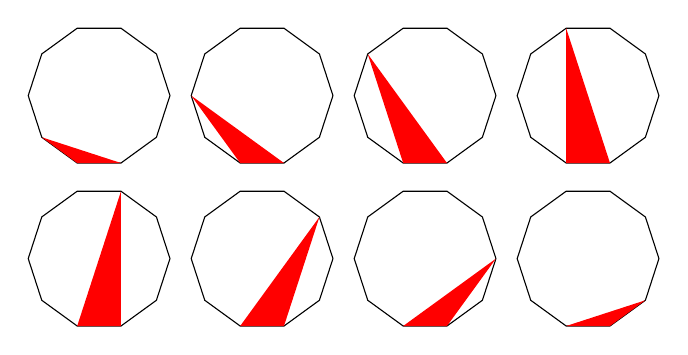
\begin{tikzpicture}
      \def\dr{2}
      \def\spc{2.3*\dr}

      \decagon{0*\spc}{\spc}{\dr}{-\dec@aii}{-\dec@bi}
      \decagon{1*\spc}{\spc}{\dr}{-1}{0}
      \decagon{2*\spc}{\spc}{\dr}{-\dec@aii}{\dec@bi}
      \decagon{3*\spc}{\spc}{\dr}{-\dec@ai}{\dec@bii}

      \decagon{0*\spc}{0}{\dr}{\dec@ai}{\dec@bii}
      \decagon{1*\spc}{0}{\dr}{\dec@aii}{\dec@bi}
      \decagon{2*\spc}{0}{\dr}{1}{0}
      \decagon{3*\spc}{0}{\dr}{\dec@aii}{-\dec@bi}
    \end{tikzpicture}
  \end{center}

  The area of each decagon is $240$.
  What is the total area of all the red triangles?
}

\def\advent@xxi@viii{
  The sum of three integers is $51$.
  The product of the same three integers is $836$. What is the product of largest integer and the second-largest integer?
}

\def\advent@xxi@ix{
  Eve writes down a sequence of consecutive positive integers (she writes more than one number).
  The sum of the numbers Eve has written down is $844$.
  Today's number is the smallest integer that Eve has written down.
}

\def\advent@xxi@x{
  Put the digits $1$ to $9$ (using each digit exactly once) in the boxes so that the sums are correct.
  Today's number is the largest number you can make using the digits in the red boxes.

  \grid@advent@xxi@x{}{}{}{}{}{}{}{}{}
}

\def\advent@xxi@xi{
  The integers are written in a triangle as shown below:
  \begin{center}
    \begin{tabular}{ccccccc}
         &    &    & 1    &    &    &    \\
         &    & 2  & 3    & 4  &    &    \\
         & 5  & 6  & 7    & 8  & 9  &    \\
      10 & 11 & 12 & 13   & 14 & 15 & 16 \\
         &    &    & etc. &    &    &
    \end{tabular}
  \end{center}
  Today's number appears directly above the number $750$ in the triangle of integers.
}

\def\advent@xxi@abgrid{
  \begin{center}
    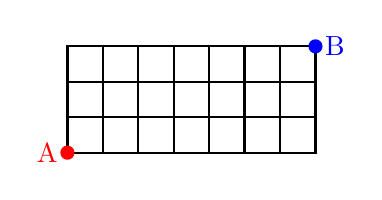
\begin{tikzpicture}
      \def\gs{1}
      % Grid
      \foreach \i in {0,...,6}{
          \foreach \j in {0,...,2}{
              \draw[thick] (\i * \gs, \j * \gs) rectangle (\i * \gs + \gs, \j * \gs + \gs);
            }
        }
      % Points
      \fill[color=red] (0, 0) circle (0.2) node[color=red,left] {A};
      \fill[color=blue] (7*\gs, 3*\gs) circle (0.2) node[color=blue,right] {B};
    \end{tikzpicture}
  \end{center}
}
\def\advent@xxi@xii{
  You start at the point marked A in the picture below. You want to get to the point marked B.
  You may travel \textbf{to the right} or \textbf{upwards} along the black lines.

  \advent@xxi@abgrid

  Today's number is the total number of possible routes to get from A to B.
}

\def\advent@xxi@xiii{
  The diagram below shows three circles and two triangles.
  The three circles all meet at one point.
  The vertices of the smaller red triangle are at the centers of the circles.
  The lines connecting the vertices of the larger blue triangle to the point where all three circles meet are diameters of the three circles.

  \begin{center}
    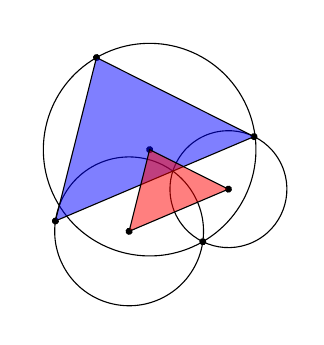
\begin{tikzpicture}[rotate=30,transform shape]
      \def\bcr{3}
      \def\scr{0.55*\bcr}
      \def\sca{34}
      \def\mcr{0.7*\bcr}
      \def\mca{142}
      \def\pr{0.1}

      % Circles
      \draw (0, \bcr) circle (\bcr);
      \draw (\sca: \scr) circle (\scr);
      \draw (\mca: \mcr) circle (\mcr);

      % Points
      \fill (0, 0) circle (\pr);
      \fill (0, \bcr) circle (\pr);
      \fill (0, 2*\bcr) circle (\pr);
      \fill (\sca: \scr) circle (\pr);
      \fill (\sca: 2*\scr) circle (\pr);
      \fill (\mca: \mcr) circle (\pr);
      \fill (\mca: 2*\mcr) circle (\pr);

      % Triangles
      \draw[fill=blue,fill opacity=0.5] (\mca: 2*\mcr) -- (0, 2*\bcr) -- (\sca: 2*\scr) -- cycle;
      \draw[fill=red,fill opacity=0.5] (\mca: \mcr) -- (0, \bcr) -- (\sca: \scr) -- cycle;
    \end{tikzpicture}
  \end{center}

  The area of the smaller red triangle is $226$.
  What is the area of the larger blue triangle?
}

\def\advent@xxi@xiv{
  You start at the point marked A in the picture below.
  You want to get to the point marked B.
  You may travel \textbf{to the right}, \textbf{upwards}, or \textbf{to the left} along the black lines, but you cannot pass along the same line segment more than once.

  \advent@xxi@abgrid

  Today's number is the total number of possible routes to get from A to B.
}

\newcommand\pyramid@advent@xxi@xvi[6]{
  \begin{center}
    \begin{tabular}{cccccc}
      (row 1) &    &    & #1   &    &    \\
      (row 2) &    & #2 &      & #3 &    \\
      (row 3) & #4 &    & #5   &    & #6 \\
              &    &    & etc. &    &
    \end{tabular}
  \end{center}
}
\def\advent@xxi@xv{
  The odd numbers are written in a pyramid.

  \pyramid@advent@xxi@xvi{1}{3}{5}{7}{9}{11}

  What is the mean of the numbers in the 19th row?
}

\newcommand\grid@advent@xxi@xvi[9]{
  \begin{center}
    \begin{tikzpicture}[scale=2]
      \gridbox{0}{2}{#1}
      \gridbox{1}{2}{#2}
      \gridbox{2}{2}{#3}
      \gridbox{0}{1}{#4}
      \gridbox{1}{1}{#5}
      \gridbox{2}{1}{#6}
      \gridbox{0}{0}{#7}
      \gridbox{1}{0}{#8}
      \gridbox{2}{0}{#9}

      % Labels
      \cwlab{0}{2}{1}
      \cwlab{1}{2}{2}
      \cwlab{2}{2}{3}
      \cwlab{0}{1}{4}
      \cwlab{0}{0}{5}
    \end{tikzpicture}
  \end{center}
}
\def\advent@xxi@xvi{
  Each clue in this crossnumber is formed of two parts connected by a logical connective: AND means that both parts are true; NAND means that at most one part is true; OR means that at least one part is true; NOR means that neither part is true; XOR means that exactly one part is true; XNOR means that either both parts are false or both parts are true.
  No number starts with $0$.

  \begin{multicols}{2}
    \grid@advent@xxi@xvi{}{}{}{}{}{}{}{}{}

    \columnbreak

    \begin{enumerate}
      \item \textbf{1A} is a palindrome XNOR \textbf{1D} is a palindrome.
      \item \textbf{1A} is greater than $350$ NOR \textbf{1D} is less than $150$.
      \item \textbf{3D} is odd NAND \textbf{4A} and \textbf{2D} are equal.
      \item \textbf{3D} is prime XOR \textbf{5A} is odd.
      \item \textbf{4A} is a cube AND \textbf{2D} is a cube.
      \item The sum of the digits of \textbf{3D} is $2$ OR the sum of the digits of \textbf{5A} is $5$.
      \item Today's number is \textbf{1D}.
    \end{enumerate}
  \end{multicols}
}

\def\advent@xxi@xvii{
  The digital product of a number is computed by multiplying together all of its digits. For example, the digital product of $6273$ is $252$.

  Today's number is the smallest number whose digital product is $252$.
}

\def\advent@xxi@xviii{
  Put the digits $1$ to $9$ (using each digit exactly once) in the boxes so that the sums are correct.
  The sums should be read left to right and top to bottom ignoring the usual order of operations.
  For example, $4 + 3 \times 2$ is $14$, not $10$.
  Today's number is the product of the numbers in the red boxes.

  \grid@advent@xxi@xviii{}{}{}{}{}{}{}{}{}
}

\def\advent@xxi@xix{
  The equation $352x^3 - 528x^2 + 90 = 0$ has three distinct real-valued solutions.

  Today's number is the number of integers $a$ such that the equation $352x^3 - 528x^2 + a = 0$ has three distinct real-valued solutions.
}

\def\advent@xxi@xx{
  What is the area of the largest area triangle that has one side of length $32$ and one side of length $19$?
}

\newcommand\grid@advent@xxi@xxi[9]{
  \begin{center}
    \begin{tikzpicture}
      \bigbox{0}{3}{#1}
      \bigbox{1}{3}{#2}
      \bigbox{2}{3}{#3}
      \bbtextr{3}{3}{\textbf{today's number}}

      \bigbox{0}{2}{#4}
      \bigbox{1}{2}{#5}
      \bigbox{2}{2}{#6}
      \bbtextr{3}{2}{prime}

      \bigbox{0}{1}{#7}
      \bigbox{1}{1}{#8}
      \bigbox{2}{1}{#9}
      \bbtextr{3}{1}{square}

      \bbtextb{0}{0}{cube}
      \bbtextb{1}{0}{odd}
      \bbtextb{2}{0}{multiple\\of $11$}
    \end{tikzpicture}
  \end{center}
}
\def\advent@xxi@xxi{
  Arrange the digits $1$–$9$ (using each digit exactly once) so that the three digit number in: the middle row is a prime number; the bottom row is a square number; the left column is a cube number; the middle column is an odd number; the right column is a multiple of $11$.
  The $3$-digit number in the first row is today's number.

  \grid@advent@xxi@xxi{}{}{}{}{}{}{}{}{}
}

\def\advent@xxi@xxii{
  There are $12$ ways of placing $2$ tokens on a $2 \times 4$ grid so that no two tokens are next to each other horizontally, vertically or diagonally:

  \begin{center}
    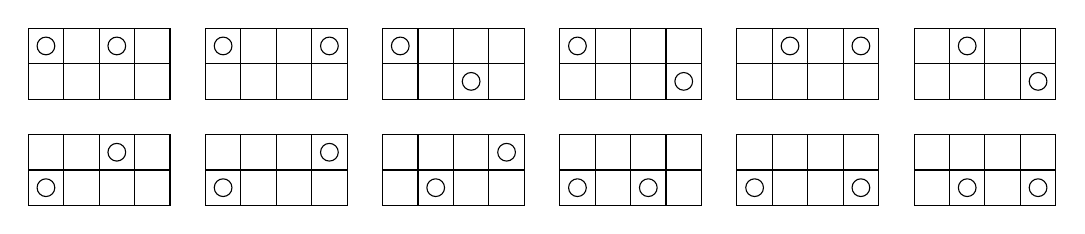
\begin{tikzpicture}
      % Draw all the grids
      \foreach \gi in {0,1}{
          \foreach \gj in {0,...,5}{
              \foreach \i in {0,1}{
                  \foreach \j in {0,...,3}{
                      \gridbox{5*\gj + \j}{3*\gi + \i}{}
                    }
                }
            }
        }

      % Place token circles
      \gridcirc{0}{4}
      \gridcirc{2}{4}
      \gridcirc{5}{4}
      \gridcirc{8}{4}
      \gridcirc{10}{4}
      \gridcirc{12}{3}
      \gridcirc{15}{4}
      \gridcirc{18}{3}
      \gridcirc{21}{4}
      \gridcirc{23}{4}
      \gridcirc{26}{4}
      \gridcirc{28}{3}
      \gridcirc{0}{0}
      \gridcirc{2}{1}
      \gridcirc{5}{0}
      \gridcirc{8}{1}
      \gridcirc{11}{0}
      \gridcirc{13}{1}
      \gridcirc{15}{0}
      \gridcirc{17}{0}
      \gridcirc{20}{0}
      \gridcirc{23}{0}
      \gridcirc{26}{0}
      \gridcirc{28}{0}
    \end{tikzpicture}
  \end{center}

  Today's number is the number of ways of placing $2$ tokens on a $2 \times 21$ grid so that no two tokens are next to each other horizontally, vertically or diagonally.
}

\def\advent@xxi@xxiii{
  I draw the parabola $y = x^2$ and mark points on the parabola at $x = 17$ and $x = -6$.
  I then draw a straight line connecting these two points.

  At which value of $y$ does this line intercept the $y$-axis?
}

\def\advent@xxi@xxiv{
  The digital product of a number is computed by multiplying together all of its digits.
  For example, the digital product of $1522$ is $20$.

  How many $12$-digit numbers are there whose digital product is $20$?
}

\def\card@xxi@i{
  What is the sum of all the odd integers between $0$ and $30$?
}

\def\card@xxi@ii{
  What is the sum of all the odd integers between $0$ and $5668$?
}

\def\card@xxi@iii{
  What is the smallest integer with a digital sum of $28$ and a digital product of $10000$?
}

\def\card@xxi@iv{
  What is the smallest integer with a digital sum of $41$ and a digital product of $432000$?
}

\def\card@xxi@v{
  What is the area of the largest area dodecagon that will fit inside a circle with area $111185 \pi$?
}

\def\card@xxi@vi{
  What is the area of the largest area heptagon that will fit inside a semicircle with area $115185 \pi$?
}

\def\card@xxi@vii{
  How many terms are there in the (simplified) expansion of $(x + y + z)^2$?
}

\def\card@xxi@viii{
  How many terms are there in the (simplified) expansion of $(x + y + z)^{41172}$?
}

\def\card@xxi@ix{
  What is the largest integer that cannot be written as $4a + 5b$ for non-negative integers $a$ and $b$?
}

\def\card@xxi@x{
  What is the largest integer that cannot be written as $83409a + 66608b$ for non-negative integers $a$ and $b$?
}

\def\card@xxi@xi{
  How many positive integers are there below $100$ whose digits are all non-zero and different?
}

\def\card@xxi@xii{
  How many positive integers are there whose digits are all non-zero and different?
}

\def\card@xxi@xiii{
  What is the only integer for which taking the geometric mean of all its factors (including $1$ and the number itself) gives $2$?
}

\def\card@xxi@xiv{
  What is the only integer for which taking the geometric mean of all its factors (including $1$ and the number itself) gives $25$?
}


\begin{document}

\title{MS Scroggs Advent Calendar 2015 Answers}
\author{Dan Whitman}
\date{}

\maketitle

Answers: \href{https://www.mscroggs.co.uk/puzzles/advent2015}{https://www.mscroggs.co.uk/puzzles/advent2015}

\aproblem{1}{200}{\advent@xv@i}{
  In general, the largest area $n$-gon that will fit in a circle is a regular $n$-gon with a circumradius equal to the radius of the circle.
  Of course, a rectangle is a quadrilateral, that is a $4$-gon, so that the largest area rectangle will actually be a square with a diagonal equal to the diameter of the circle.
  A square with sides $s$ has an area $A = s^2$ and a diagonal of $d = \sqrt{2}s$ so that of course $s = d / \sqrt{2}$.
  We have a circle of radius $r = 10$ so that the diameter is of course $2r$.
  The area of the square is thus
  \gath{
    A = s^2 = \parens{\frac{d}{\sqrt{2}}}^2 = \frac{d^2}{2} = \frac{(2r)^2}{2} = \frac{4r^2}{2} = 2r^2 = 2 \cdot 10^2 = 200 \,,
  }
  which is our answer.
}

\aproblem{2}{154}{\advent@xv@ii}{
  Consider a twelve hour period from 12:01 to 12:01.
  The minute hand aligns with the hour hand first between 1:00 and 2:00 (precisely at 1:05), and then between 2:00 and 3:00 (at exactly 2:10), and lastly at exactly 12:00.
  This is $11$ times once the clock strikes the next 12:01.
  Hence during a day starting at 12:01 (i.e. two $12$ hour periods) this happens $22$ times.
  So, during a week, this happens $7 \cdot 22 = 154$ times.
}

\aproblem{3}{304}{\advent@xv@iii}{
  The answer is just from the blog post.
  Since the number exploits symmetry and the fact that games are ended once a player wins, deriving this number analytically or even using a Python program would be highly non-trivial.
}

\aproblem{4}{108}{\advent@xv@iv}{
  \boxans{\grid@advent@xv@iv{1}{9}{4}{2}{7}{5}{3}{8}{6}}
}

\aproblem{5}{208}{\advent@xv@v}{
  For a triangle to be valid, the pairwise sum of the lengths of two sides must be strictly greater than the third side.
  So suppose we have potential sides $a$, $b$, and $c$ such that
  \gath{
    0 < a \leq b \leq c \,. \label{eqn:05:ineq}
  }
  We always have
  \gath{
    b > 0 \non
    b + c > c \geq a
  }
  and
  \gath{
    a > 0 \non
    a + c > c \geq b \,.
  }
  Therefore, for $a$, $b$, and $c$ that meet \eqref{eqn:05:ineq}, these can form the sides of a valid triangle if and only if
  \gath{
    a + b > c \,. \label{eqn:05:cond}
  }
  The perimeter of the triangle is of course $p = 100 = 2k = a + b + c$ when $k = 50$, and we are only interested in triangles with this perimeter.
  Hence
  \gath{
    a + b > c \non
    p - c > c \non
    2k > 2c \non
    c < k \,,
  }
  that is, in order for \eqref{eqn:05:cond} to be met so that the triangle is valid, it must be that $c < k = 50$.
  Now, suppose that $c = k - r$ where $r \geq 1$ is an integer.
  Also suppose that $b = c - s = k - r - s$ where $s \geq 0$ is an integer.
  This of course ensures that $b \leq c$ per \eqref{eqn:05:ineq}.
  Then set $a = 2r + s$ so that
  \gath{
    a + b + c = (2r + s) + (k - r - s) + (k - r) = 2r + s + 2k - 2r - s = 2k = p
  }
  just as we require.
  To enforce $a \leq b$, we get
  \gath{
    2r + s \leq k - r - s \non
    2s \leq k - 3r \non
    0 \leq s \leq \floor{\frac{k - 3r}{2}}
  }
  since $s$ must be an integer.
  Thus the number of valid triangles for a given $r$ is
  \gath{
    N(r) = \floor{\frac{k - 3r}{2}} + 1
  }
  since $s$ can be zero.
  The largest that $r$ can be so that $s$ is valid is such that $f(r) = \floor{(k - 3r)/2}$ is as low as possible, but no lower than zero.
  Since $k \equiv 2 \pmod{3}$ for our $k = 50$, this is $r = 16$, for which $f(16) = 1$, noting that $f(17) = -1$, which is going too far.
  Thus the total number of valid triangles with integer sides is
  \gath{
    N = \sum_{r=1}^{16} N(r) = \sum_{r=1}^{16} \parens{\floor{\frac{k - 3r}{2}} + 1} \,,
  }
  which is difficult to evaluate analytically due to the floor function.
  However, this can be evaluated if we break it up into two cases.
  First, note that $k = 50$ is even and so $k = 2l$ for $l = 25$.
  Now, if $r$ is even then $r = 2n$ for some $n$ so that
  \gath{
    N(2n) = \floor{\frac{k - 3r}{2}} + 1 = \floor{\frac{2l - 3(2n)}{2}} + 1 = \floor{\frac{2(l - 3n)}{2}} + 1 = l - 3n + 1 \,.
  }
  On the other hand, if $r$ is odd, then $r = 2n-1$ for some $n$ so that
  \ali{
    N(2n-1) &= \floor{\frac{k - 3r}{2}} + 1 = \floor{\frac{2l - 3(2n-1)}{2}} + 1 = \floor{\frac{2l - 6n + 3}{2}} + 1 \non
    &= \floor{\frac{2l - 6n + 2 + 1}{2}} + 1 = \floor{\frac{2(l - 3n + 1) + 1}{2}} + 1 \non
    &= \floor{(l - 3n + 1) + \frac{1}{2}} + 1 = (l - 3n + 1) + 1 \non
    &= l - 3n + 2 \,.
  }
  Therefore, since $16 = 2 \cdot 8$, it follows that
  \ali{
    N &= \sum_{r=1}^{16} N(r) = \sum_{n=1}^8 \squares{N(2n) + N(2n-1)} = \sum_{n=1}^8 \squares{(l - 3n + 1) + (l - 3n + 2)} \non
    &= \sum_{n=1}^8 \squares{2l - 6n + 3} = 16l - 6\sum_{n=1}^8 n + 24 = 16l - 6 \frac{8 \cdot 9}{2} + 24 \non
    &= 16l - 216 + 24 = 16l - 192 \non
    &= 16 \cdot 25 - 192 =  208 \,,
  }
  which is our answer.
  This was verified against a brute force Python program.
}

\aproblem{6}{385}{\advent@xv@vi}{
  \boxans{\grid@advent@xv@vi{3}{8}{5}{4}{9}{7}{2}{1}{6}}
}

\aproblem{7}{138}{\advent@xv@vii}{
  Let $N(n)$ denote the number of ways that integer $n$ can be calculated as a linear combination of $3$ (penalty kick or drop goal), $5$ (try), and $7$ (try and conversion).
  A brute force Python function was written to calculate $N(n)$ for a given $n$.
  Then we calculate this for increasing $n$ until we find three consecutive $n$, $n+1$, and $n+2$ for which the number of ways is greater than our desired $101$ ways.
  We go back and look for the largest $k < n$ such that $N(k) = 101$.
  We are then guaranteed that $k$ is the highest integer such that $N(k) = 101$.
  This is because $n$, $n+1$, and $n+2$ must cover all three values modulo $3$, and so for any number higher than $n+2$, say $m$, it must congruent to one of these modulo $3$, say $n+l$ for $0 \leq l \leq 2$.
  Then of course $m = n+l + 3r$ for some $r$ so that
  \gath{
    N(m) \geq N(n+l) > 101 \,.
  }
}

\aproblem{8}{720720}{\advent@xv@viii}{
  The number $720720$ has $240$ factors, which was determined by a brute force Python program.
}

\aproblem{9}{792}{\advent@xv@ix}{
  Let $N(h, w)$ denote the number of routes from the lower left corner of a $h \times w$ (height by width) grid to the upper right corner.
  In our case we are looking for $N(5, 7)$, which we can first deduce by considering the number of spaces below and to the right of the route.
  In the bottom row, the spaces to the right of the route can be any number from $0$ (if the route goes along the entire bottom and then up the right side) to $7$ (if the route starts by going immediately up from A).
  Then, \emph{for each} of the number of spaces to the right of the route in the first (i.e. bottom) row $a_1$, the number of spaces to the right of the route in the second row $a_2$ can be any number from $0$ to $a_1$, i.e. the route runs to the right along the top of the first row then goes up at the node where $a_2$ spaces are to the right in the second row.
  This applies in the same way to the third  row based on $a_2$ and so on.
  As these possibilities must be added the number of routes for a $5 \times w$ grid can be expressed as
  \ali{
    N(5, w) &= \sum_{a=0}^w \sum_{b=0}^a \sum_{c=0}^b \sum_{d=0}^c \sum_{e=0}^d 1 = \sum_{a=0}^w \sum_{b=0}^a \sum_{c=0}^b \sum_{d=0}^c (d + 1) = \sum_{a=0}^w \sum_{b=0}^a \sum_{c=0}^b \sum_{d=1}^{c+1} d \non
    &= \sum_{a=0}^w \sum_{b=0}^a \sum_{c=0}^b \frac{(c+1)(c+2)}{2} = \frac{1}{2} \sum_{a=0}^w \sum_{b=0}^a \sum_{c=0}^b (c^2 + 3c + 2) \non
    &= \frac{1}{2} \sum_{a=0}^w \sum_{b=0}^a \squares{\sum_{c=0}^b c^2 + 3 \sum_{c=0}^b c + 2\sum_{c=0}^b 1} = \frac{1}{2} \sum_{a=0}^w \sum_{b=0}^a \squares{\frac{2b^3 + 3b^2 + b}{6} + 3\frac{b^2 + b}{2} + 2(b+1)} \non
    &= \frac{1}{12} \sum_{a=0}^w \sum_{b=0}^a \squares{2b^3 + 3b^2 + b + 9b^2 + 9b + 12b + 12} = \frac{1}{6} \sum_{a=0}^w \sum_{b=0}^a \squares{b^3 + 6b^2 + 11b + 6} \non
    &= \frac{1}{6} \sum_{a=0}^w \squares{\sum_{b=0}^a b^3 + 6 \sum_{b=0}^a b^2 + 11 \sum_{b=0}^ab + 6 \sum_{b=0}^a 1} \non
    &= \frac{1}{6} \sum_{a=0}^w \squares{\frac{a^4 + 2a^3 + a^2}{4} + 6\frac{2a^3 + 3a^2 + a}{6} + 11\frac{a^2 + a}{2} + 6(a+1)} \non
    &= \frac{1}{24} \sum_{a=0}^w \squares{a^4 + 2a^3 + a^2 + 8a^3 + 12a^2 + 4a + 22a^2 + 22a + 24a + 24} \non
    &= \frac{1}{24} \sum_{a=0}^w \squares{a^4 + 10a^3 + 35a^2 + 50a + 24} \non
    &= \frac{1}{24} \squares{\sum_{a=0}^w a^4 + 10 \sum_{a=0}^w a^3 + 35 \sum_{a=0}^w a^2 + 50 \sum_{a=0}^w a + 24\sum_{a=0}^w 1} \non
    &= \frac{1}{24} \squares{\frac{6w^5 + 15w^4 + 10w^3 - w}{30} + 10 \frac{w^4 + 2w^3 + w^2}{4} + 35 \frac{2w^3 + 3w^2 + w}{6} + 50 \frac{w^2 + w}{2} + 24(w+1)} \non
    &= \frac{1}{1440} \left[12w^5 + 30w^4 + 20w^3 - 2w + 150w^4 + 300w^3 + 150w^2 + 700w^3 + 1050w^2 + 350w \right. \non
      &\mlesp \left.+ 1500w^2 + 1500w + 1440w + 1440\right] \non
    &= \frac{1}{1440} \squares{12w^5 + 180w^4 + 1020w^3 + 2700w^2 + 3288w + 1440} \non
    &= \frac{1}{120} \squares{w^5 + 15w^4 + 85w^3 + 225w^2 + 274w + 120} \,.
  }
  When we plug in our $w = 7$ we get our answer $N(5, 7) = 792$.
  We can also solve this problem using a recursive function, which is more difficult to calculate analytically, but easier to implement on a computer.
  For simplicity, we change our convention so that the upper right corner is node $(0, 0)$ and other nodes are numbered $(y, x)$, where $y$ increases downward, and $x$ increases to the left.
  Thus the lower left corner becomes $(h, w)$, though $N(h, w)$ retains its original meaning.
  In our base case we have that that $N(h, 0) = N(0, w) = 1$ for any $h$ and $w$, which is due to the fact that, once the top or right side of the total grid is reached, there is only one way to complete the journey to the upper right corner.
  Then, at a node $(y, x)$, the number of routes to get from this node to the upper right corner is
  \gath{
    N(y, x) = N(y-1, x) + N(y, x-1) \,,
  }
  which is the sum of the number of routes if we go up and the number of routes if we instead go right.
  This simple recursive function was implemented in Python and was found to give the same answer as above for $N(5, 7)$.
}

\aproblem{10}{788}{\advent@xv@x}{
  If $x$ is our unknown number, then the question translates to the following system of modulo congruencies:
  \ali{
    x &\equiv 0 \pmod{2} \label{eqn:10:first} \\
    x \equiv -1 &\equiv 2 \pmod{3} \\
    x \equiv -2 &\equiv 3 \pmod{5} \\
    x \equiv -3 &\equiv 4 \pmod{7} \\
    x \equiv -4 &\equiv 7 \pmod{11} \\
    x \equiv -5 &\equiv 8 \pmod{13} \label{eqn:10:last}
  }
  Since clearly the moduli $m_1=2$, $m_2=3$, $m_3=5$, $m_4=7$, $m_5=11$, and $m_6=13$ are all prime, they are pairwise coprime, and so we can use the Chinese Remainder Theorem and the Euclidean algorithm to solve it.
  The first step in this is to find multiplicative inverses $h_i$ for $M_i$ modulo $m_i$, where $M_i$ is the product of all the moduli except $m_i$.
  That is, if $M$ is the product of all the moduli, then $M_i = M / m_i$.
  This can be done with the Euclidean algorithm, but since the moduli are small, we just find them by trial and error:
  \begin{center}
    \begin{tabular}{cccc}
      $m_i$ & $M_i$ & $M_i \pmod{m_i}$ & $h_i$ \\
      \hline
      $2$ & $15015$ & $1$ & $1$ \\
      $3$ & $10010$ & $2$ & $2$ \\
      $5$ & $6006$ & $1$ & $1$ \\
      $7$ & $4290$ & $6$ & $6$ \\
      $11$ & $2730$ & $2$ & $6$ \\
      $13$ & $2310$ & $9$ & $3$
    \end{tabular}
  \end{center}
  There are then an infinite number of solutions where $x$ is a solution if and only if
  \gath{
    x \equiv \sum_{i=1}^6 x_i M_i h_i \pmod{M} \,, \label{eqn:10:x}
  }
  where each $x_i$ is what $x$ is congruent to modulo $m_i$ as in \eqref{eqn:10:first} through \eqref{eqn:10:last}. For example $x_2 = 2$, $x_4 = 4$, and $x_6 = 8$.
  For our numbers in the table above, \eqref{eqn:10:x} evaluates to
  \gath{
    x \equiv 788 \pmod{30030} \,.
  }
  Evidently the answer is the lowest positive value that satisfies this, that is $788$.
  This was verified to satisfy the original conditions with Python.
}

\aproblem{11}{742}{\advent@xv@xi}{
  We know that this is a three-digit number, so suppose that our number has the digits $d_2 d_1 d_0$.
  With what was given in the problem, we have that
  \gath{
    100 d_2 + 10 d_1 + d_0 = 3\parens{100 d_0 + 10 d_1 + d_2} + 1 = 300 d_0 + 30 d_1 + 3 d_2 + 1 \non
    97 d_2 - 1 = 299 d_0 + 20 d_1 \label{eqn:11:e}
  }
  Now, all the digits can be from $0$ to $9$, and so, letting $f(x) = 97x - 1$, we have the following possible values for the left side of \eqref{eqn:11:e}:
  \begin{center}
    \begin{tabular}{c|ccc}
      $d_2$ & $f(d_2)$ & $f(d_2) \pmod{299}$ & $f(d_2) \pmod{20}$ \\
      \hline
      \rowcolor{lightgray} 0 & -1 & 298 & 19 \\
      \rowcolor{lightgray} 1 & 96 & 96 & 16 \\
      \rowcolor{lightgray} 2 & 193 & 193 & 13 \\
      \rowcolor{lightgray} 3 & 290 & 290 & 10 \\
      4 & 387 & 88 & 7 \\
      5 & 484 & 185 & 4 \\
      6 & 581 & 282 & 1 \\
      7 & 678 & 80 & 18 \\
      8 & 775 & 177 & 15 \\
      9 & 872 & 274 & 12 \\
    \end{tabular}
  \end{center}
  As none of these are divisible by either $299$ or $20$, this means that neither $d_0$ nor $d_1$ can be zero, which is unfortunate as this would accelerate the solution.
  Since $d_0 > 0$, that means that both sides of the equation must be no less than $299$ so that we can remove from consideration the first four rows of the above table (hence why they are grayed).
  Now since the maximum that $d_2$ can be is $9$, the maximum that both sides of the equation can be is $872$.
  Hence it must be that $1 \leq d_0 \leq 2$ (i.e. $d_0$ must be $1$ or $2$) since $299 d_0 \geq 897 > 872$ when $d_0 \geq 3$ so that this also applies to the entire right side.
  Supposing that $d_0 = 1$, then we have:
  \gath{
    97 d_2 - 1 = 299 \cdot 1 + 20 d_1 \non
    97 d_2 - 300 = 20 d_1 \,.
  }
  Below, the positive possible values of the left side are then:
  \begin{center}
    \begin{tabular}{c|ccc}
      $d_2$ & $97 d_2 - 300$ \\
      \hline
      4 & 88 \\
      5 & 185 \\
      6 & 282 \\
      7 & 379 \\
      8 & 476 \\
      9 & 573 \\
    \end{tabular}
  \end{center}
  Since none the these are divisible by $20$, it must be that $d_0 = 2$.
  This means that
  \gath{
    97 d_2 - 1 = 299 \cdot 2 + 20 d_1 \non
    97 d_2 - 599 = 20 d_1\,,
  }
  and we also have the positive possible values for the left side as
  \begin{center}
    \begin{tabular}{c|ccc}
      $d_2$ & $97 d_2 - 599$ \\
      \hline
      7 & 80 \\
      8 & 177 \\
      9 & 274 \\
    \end{tabular}
  \end{center}
  Therefore $d_2 = 7$ since this is the only value for which the left side is divisible by $20$.
  Clearly also then $d_1 = 4$ since then $20 d_1 = 20 \cdot 4 = 80$.
  Hence our answer is $d_2 d_1 d_0 = 742$.
  That this satisfies the original requirement was verified with Python.
}

\aproblem{12}{252}{\advent@xv@xii}{
  \boxans{\grid@advent@xv@xii{3}{1}{6}{7}{9}{4}{8}{2}{5}}
}

\aproblem{13}{729}{\advent@xv@xiii}{
  \boxans{\grid@advent@xv@xiii{1}{5}{7}{4}{8}{2}{6}{3}{9}}
}

\aproblem{14}{313}{\advent@xv@xiv}{
  This was solved using a brute force Python program, since it likely would have to be solved with a manual search anyway.
}

\aproblem{15}{328}{\advent@xv@xv}{
  There is no easy way to solve this analytically, but the following algorithm will calculate it.
  First define the set $A = \braces{1,2,3,4,5,6,7}$ and, for a positive integer $n$, let $B(n)$ be the subset of $A$ such that $k \in B(n)$ if and only if $k > n$ or $k$ is a factor of $n$.
  Now we define a recursive function $f(n, R)$, where $n \in A$ is the previous number in the sequence, $R \subseteq A$ are the remaining numbers to place, and the return value of $f$ is the number of valid ways to arrange the remaining numbers $R$ in an arrangement that starts with $n$.
  We then have the following cases and return values that define the recursive $f(n, R)$:

  Case: $R$ is empty. The arrangement is complete, so return $1$.

  Case: If $R$ is nonempty but $B(n)$ is empty then there are no valid ways to complete this arrangement, so return $0$.

  Case: If $R$ and $B(n)$ are both nonempty, then return
  \gath{
    \sum_{k \in B(n) \cap R} f(k, R - \braces{k}) \,.
  }

  Since the first number in the arrangement can be any $n \in A$, our answer is then
  \gath{
    \sum_{n \in A} f(n, A - \braces{n}) \,.
  }
  This recursive function was implemented in Python, giving us our answer $328$.
}

\aproblem{16}{685}{\advent@xv@xvi}{
  First let $x_1 = 729$, $x_2 = 313$, and $x_3 = 328$ be the known answers for the Dec~$13$th, $14$th, and $15$th problems, respectively.
  If $a$ is the answer to today's problem, then, by what is given we have that
  \gath{
    a = \frac{4}{3} \cdot \frac{1}{4} \parens{\sum_{i=1}^3 x_i + a} \non
    a = \frac{1}{3} \parens{\sum_{i=1}^3 x_i + a} \non
    3a = \sum_{i=1}^3 x_i + a \non
    2a = \sum_{i=1}^3 x_i \non
    a = \frac{1}{2} \sum_{i=1}^3 x_i = \frac{1}{2} \parens{729 + 313 + 328} = \frac{1370}{2} = 685 \,.
  }
  That this answer verifies the original condition was verified with Python.
}

\aproblem{17}{205}{\advent@xv@xvii}{
  The number of zeros at the end of a number is the same as the number of \mn{10} in the product that makes the number.
  Each of these \mn{10} is made by multiplying a $5$ and a $2$.
  There will clearly be many more even numbers than multiples of $5$ in any large number, and so plenty of \mn{2} to pair with each $5$.
  Hence the number of \mn{5} will tell us how many zeros the number ends in.
  Because of this, for a general positive integer $n$, $n!$ will end in $f(n)$ zeros where
  \gath{
    f(n) = \sum_{i=1}^\infty \floor{\frac{n}{5^i}} \,.
  }
  Of course eventually the terms will all be zero once $5^i$ becomes larger than $n$.
  Now, we know that $n < 5 \cdot 50 = 250$ since $f(250) > 250/5 = 50$, and thus $5^3 = 125$ is the largest power of $5$ we need to worry about since $5^4 = 625 > 250 > n$.
  We can get close to our answer if we solve
  \gath{
    \frac{n}{5} + \frac{n}{25} + \frac{n}{125} = 50 \non
    25n + 5n + n = 50 \cdot 125 = 6250 \non
    31n = 6250 \non
    n \approx 201.6
  }
  However, we have $f(201) = 40 + 8 + 1 = 49$, so we are not quite there.
  If we increase this to $n = 205$ then we get one extra factor of $5$ in there with no additional factors of $25$ or $125$, hence  $f(205) = 41 + 8 + 1 = 50$ so that $n = 205$ is our answer.
  This was verified by brute force with Python, which supports arbitrarily large integers so that factorials can actually be evaluated and the zeros counted.
}

\aproblem{18}{834}{\advent@xv@xviii}{
  \boxans{\grid@advent@xv@xviii{8}{9}{1}{3}{7}{2}{4}{6}{5}}
}

\aproblem{19}{147}{\advent@xv@xix}{
  There does not seem to be an easy way to solve this analytically, but we can design a recursive algorithm to count the possible ways.
  We consider sequences of positive integer denominators $\angles{n_i}$ such that each term in the sum is $1/n_i$.
  Since the order of the sequence does not affect the sum, we only consider sequences $\angles{n_i}$ that are non-decreasing, that is $n_i \leq n_j$ whenever $i < j$.
  Now suppose we have chosen $k$ fractions so far and $m$ remain (so that in our case $k + m = 5$).
  Then the sum so far is
  \gath{
    s = \sum_{i=1}^k \frac{1}{n_i}
  }
  so that the remaining fractions must sum to $1 - s$.
  Since we are only considering non-decreasing sequences, the remaining $n_i$ can be no smaller than $n_k$, and so the \emph{largest} any remaining term can be is $1/n_k$.
  Hence the largest that the sum of the remaining terms can be is $m / n_k$ if all the remaining terms are $1/n_k$.
  Therefore, for the next $n_{k+1}$, we have
  \gath{
    1 - s \leq \frac{m}{n_{k+1}} \non
    n_{k+1}(1 - a) \leq m \non
    n_{k+1} \leq \frac{m}{1 - s} \,,
  }
  noting that $1 - s$ will be positive.
  Since $m / (1 - s)$ may not always be an integer, we can limit $n_{k+1}$ by
  \gath{
    n_k \leq n_{k+1} \leq \floor{\frac{m}{1 - s}} \,.
  }
  Now we define a recursive function $N(m, n, s)$ that is the number of unit fraction sums that add to $1$ where $m$ is the number of terms remaining in the sum, $1/n$ is last term in the sum so far, and $s$ is the sum so far:

  Case: $m = 0$.
  The sequence is complete since there are no remaining terms.
  If the sum $s = 1$, then this is a valid sequence so return $1$.
  Otherwise the sequence is invalid so return $0$.

  Case: $m > 0$ and $s \geq 1$.
  The sum has gone over $1$ (or is prematurely $1$) so that this sequence is already invalid, hence return $0$.

  Case: $m > 0$ and $s < 1$.
  The sequence is incomplete but still potentially valid, and so we recurse.
  In particular, we return
  \gath{
    \sum_{i = n}^{\floor{m/(1-s)}} N(m - 1, i, s + 1/i)
  }
  Since clearly the very first term in the sum cannot be $1/1 = 1$ (since then the sum would exceed $1$), the smallest possible initial denominator is $2$.
  Therefore our answer results from recursively evaluating $N(5, 2, 0)$.
  Implementing and executing this algorithm in Python gives our answer $N(5, 2, 0) = 147$.
}

\aproblem{20}{TODO}{\advent@xv@xx}{
  TODO
}

\aproblem{21}{TODO}{\advent@xv@xxi}{
  TODO
}

\aproblem{22}{TODO}{\advent@xv@xxii}{
  TODO
}

\aproblem{23}{TODO}{\advent@xv@xxiii}{
  TODO
}

\aproblem{24}{TODO}{\advent@xv@xxiv}{
  TODO
}

\end{document}
